\chapter{Graphen}

Ein Graph ist eine Struktur, die verwendet wird, um Beziehungen zwischen Objekten darzustellen.
Die Idee, Objekte durch Verbindungen zu verknüpfen, bildet die Grundlage für viele Anwendungen, unter anderem für die Routenplanung.
Graphen und (kürzeste) Pfade spielen darüber hinaus eine wichtige Rolle; in einem Wissensgraphen kann ein Pfad beispielsweise dafür stehen, dass eine Aussage wahr ist.
\autoref{graphs:fig:beispielgraph} zeigt einen Graphen, welcher im folgenden für Beispiele benutzt wird.

\begin{figure}[ht]
    \centering
    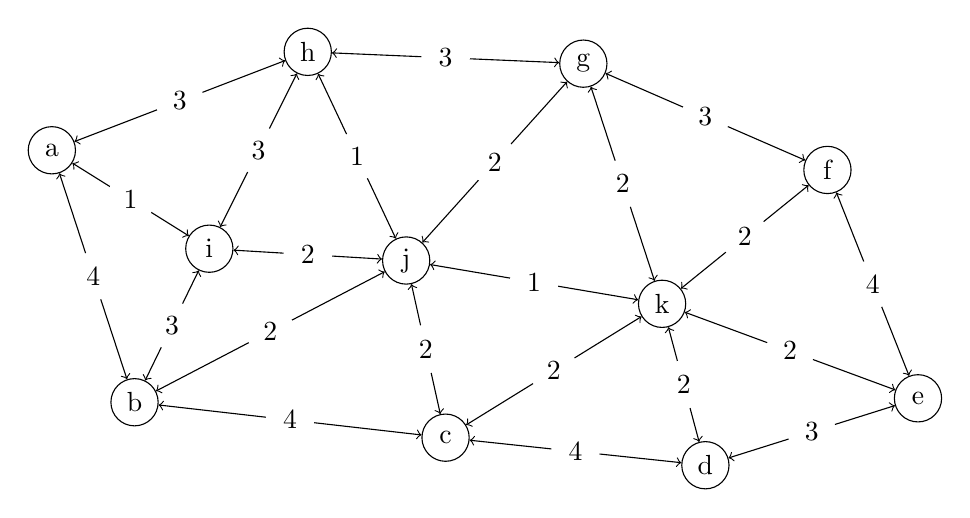
\begin{tikzpicture}
        % Nodes
        \node[circle, draw, minimum size=0.6cm, inner sep=0pt] at (0.5* 0.0, 0.5* 8.5)  (a)    {a};
        \node[circle, draw, minimum size=0.6cm, inner sep=0pt] at (0.5* 2.1, 0.5* 2.1)  (b)    {b};
        \node[circle, draw, minimum size=0.6cm, inner sep=0pt] at (0.5* 10.0, 0.5* 1.2)  (c)    {c};
        \node[circle, draw, minimum size=0.6cm, inner sep=0pt] at (0.5* 16.6, 0.5* 0.5)  (d)    {d};
        \node[circle, draw, minimum size=0.6cm, inner sep=0pt] at (0.5* 22.0, 0.5* 2.2)  (e)    {e};
        \node[circle, draw, minimum size=0.6cm, inner sep=0pt] at (0.5* 19.7, 0.5* 8.0)  (f)    {f};
        \node[circle, draw, minimum size=0.6cm, inner sep=0pt] at (0.5* 13.5, 0.5* 10.7)  (g)    {g};
        \node[circle, draw, minimum size=0.6cm, inner sep=0pt] at (0.5* 6.5, 0.5* 11.0)  (h)    {h};
        \node[circle, draw, minimum size=0.6cm, inner sep=0pt] at (0.5* 4.0, 0.5* 6.0)  (i)    {i};
        \node[circle, draw, minimum size=0.6cm, inner sep=0pt] at (0.5* 9.0, 0.5* 5.7)  (j)    {j};
        \node[circle, draw, minimum size=0.6cm, inner sep=0pt] at (0.5* 15.5, 0.5* 4.6)  (k)    {k};


        \draw[<->]  (a) edge node[circle, fill=white] {4} (b);
        \draw[<->]  (a) edge node[circle, fill=white] {3} (h);
        \draw[<->]  (a) edge node[circle, fill=white] {1} (i);

        \draw[<->]  (b) edge node[circle, fill=white] {4} (c);
        \draw[<->]  (b) edge node[circle, fill=white] {3} (i);
        \draw[<->]  (b) edge node[circle, fill=white] {2} (j);

        \draw[<->]  (c) edge node[circle, fill=white] {4} (d);
        \draw[<->]  (c) edge node[circle, fill=white] {2} (j);
        \draw[<->]  (c) edge node[circle, fill=white] {2} (k);

        \draw[<->]  (d) edge node[circle, fill=white] {3} (e);
        \draw[<->]  (d) edge node[circle, fill=white] {2} (k);

        \draw[<->]  (e) edge node[circle, fill=white] {4} (f);
        \draw[<->]  (e) edge node[circle, fill=white] {2} (k);

        \draw[<->]  (f) edge node[circle, fill=white] {3} (g);
        \draw[<->]  (f) edge node[circle, fill=white] {2} (k);

        \draw[<->]  (g) edge node[circle, fill=white] {3} (h);
        \draw[<->]  (g) edge node[circle, fill=white] {2} (j);
        \draw[<->]  (g) edge node[circle, fill=white] {2} (k);

        \draw[<->]  (h) edge node[circle, fill=white] {3} (i);
        \draw[<->]  (h) edge node[circle, fill=white] {1} (j);

        \draw[<->]  (i) edge node[circle, fill=white] {2} (j);

        \draw[<->]  (j) edge node[circle, fill=white] {1} (k);
    \end{tikzpicture}
    \caption{Beispielgraph}
    \label{graphs:fig:beispielgraph}
\end{figure}

\section{Definitionen}
Damit in den nachfolgenden Kapiteln sinnvoll argumentiert werden kann, führen wir ein paar Grundlegende Begriffe ein.

\begin{definition}[Graph]
    Sofern nicht anders angegeben, bezeichnet Graph im Folgenden einen endlichen, gerichteten Graphen mit Kantengewichten ohne Mehrfachkanten und Schleifen.

    Als Schreibweise wird $G = (V, E)$ verwendet, wobei $V$ die Knotenmenge und $E$ die Kantenmenge ist. Eine Kante ist hierbei ein Tupel $(t, h, w)$. Man bezeichnet $t \in V$ als \emph{Fuß} (Tail), $h \in V$ als \emph{Kopf} (Head) und $w \in \mathbb{R}^+$ als \emph{Gewicht} (Weight). Gelegentlich wird auch nur $(t, h)$ geschrieben, um auszudrücken, dass zwei Knoten verbunden sind.

    Wird $G$ als ungerichtet bezeichnet, so gilt $(t, h, w) \in E \Leftrightarrow (t, h, w)^T \coloneq (h, t, w) \in E$ und $(t, h)$ kann als $\{ t, h \}$ geschrieben werden.
\end{definition}

Das Gewicht der Kanten ist hierbei auf positive reelle Zahlen begrenzt, da das Verwenden eines Kantengewichtes $0$ dazu führen kann, dass ein kürzester Pfad mehrfach einen Teilpfad der Länge 0 durchläuft.
Negative Kantengewichte erschweren die Definition und Argumentation, sodass hier auf diese nicht weiter eingegangen wird.

\begin{definition}[Nachbar]
    Sei $G = (V, E)$. Ein Knoten $u \in V$ heißt \emph{Vorgänger} eines Knoten $v \in V$ wenn $(u, v) \in E$. $v$ ist dann ein \emph{Nachfolger} von $u$.
    Ist $G$ ungerichtet, so spricht man in beiden Fällen von \emph{Nachbarn}.
\end{definition}

Die Anzahl der Nachbarn eines Knotens wird als sein \emph{Grad} bezeichnet, wobei bei gerichteten Graphen vom \emph{Eingangsgrad} und \emph{Ausgangsgrad} gesprochen wird.
Hat ein Knoten keine Vorgänger oder Nachfolger, so nennt man ihn \emph{isoliert}.

\begin{definition}[Pfad]
    Ein Pfad $p$ auf einem Graph $G = (V, E)$ ist eine Folge von Knoten $(v_1, \dotsc, v_n)$, für die gilt, die benachbarte Knoten $v_i$ und $v_{u+1}$ im Pfad durch eine Kante in $G$ verbunden sind.
    Der Knoten $v_1$ wird Startknoten, $v_n$ Zielknoten genannt.
    Die Summe der Kantengewichte aller Kanten $(v_i, v_{i + 1})$ wird \emph{Länge}, die Anzahl der Kantennutzungen ($n - 1$) \emph{Hop-Länge}, genannt.
\end{definition}

Häufig wird für den Startknoten der Buchstabe $s$ (Source) und für den Zielknoten der Buchstabe $t$ (Target) verwendet.
Zwischen zwei Knoten kann es Pfade unterschiedliche Länge geben, dies führt zur Definition des kürzesten Pfades.

\begin{definition}[Kürzester Pfad]
    Ein Pfad $p$ ist \emph{ein kürzester Pfad}, wenn die Länge von $p$ unter allen Pfaden von $v_1$ nach $v_n$ minimal ist.
    Die Länge des kürzesten Pfades wird als \emph{Abstand} von $v_1$ und $v_n$ bezeichnet.

    Die Funktion ${spd} \colon V \times V \to \mathbb{R}^+ \cup \{ \infty \} $ (shortest path distance) weist einem Knotenpaar den Abstand zu, wobei dieser unendlich ist, wenn kein Pfad zwischen ihnen existiert.
    Sei nun $P \subset V \times V$ die Menge der Knoten, zwischen denen ein Pfad existiert.
    Dann weist ${sp} \colon P \to V \times V \times \dots \times V$ (shortest path) einem Knotenpaar einen kürzesten Pfad zu.
\end{definition}

Die zu beantwortende Frage, ob es zwischen zwei Knoten $s, t \in V$ einen Pfad gibt und was der Abstande der Knoten ist, bezeichnet man auch als $s-t$ Query und einen gefunden Pfad asl $s-t$ Pfad.
Zusätzlich zum Finden eines Pfades zwischen zwei Knoten ist es häufig notwendig die kürzesten Pfade von einem Knoten zu allen anderen Knoten zu finden.
Auch die Umkehrung dieses Problem ist Interessant, also die kürzesten Pfade von allen Knoten zu einem Anderen zu bestimmen.
Diese Probleme sind äquivalent, da das Finden aller kürzesten Pfade zu einem Knoten auf einem Graph $G$ dem Finden aller kürzester Pfade auf dem Umkehrgraph $G^T$ entspricht.

\begin{definition}[Transponierter Graph]
    Sei $G = (V, E)$ ein Graph. Dann ist $G^T \coloneq (V, E^T)$ mit $(t, h, w) \in E \Leftrightarrow (h, t, w) \in E^T$ der \emph{transponierte Graph} von $G$.
\end{definition}

Ein ungerichteter Graph ist hierbei selbst sein transponierter Graph.

\begin{definition}[Hitting-Set]
    Sei $G = (V, E)$ ein Graph und $P$ eine Menge an Pfaden auf $G$.
    Ein Hitting-Set $H \subset V$ ist eine Menge an Knoten, in der jeder Pfad $p \in P$ mindestens einen Knoten aus $H$ enthält.
\end{definition}

Ein triviales Beispiel für ein Hitting-Set ist $V$ selbst, im Weiteren sind jedoch möglichst kleine Hitting-Sets nützlich.
Das Finden kleinst möglicher Hitting-Sets ist NP-vollständig \cite{Kar72}.
Der Greedy-Algorithmus \ref{graphs:alg:greedy-hitting-set} bietet jedoch eine Approximation in polynomieller Zeit an.

\begin{algorithm}
    \caption{Greedy Hitting-Set}
    \begin{algorithmic}[1]
        \Require Knotenmenge $V$, Pfade $P$ über $V$
        \Ensure Hitting-Set $H$

        \State $H \gets \emptyset$

        \State

        \While{$P \neq \emptyset$}
        \State Wähle $v \in V$ mit $\abs{ \{ p \mid p \in P \colon v \in p \}}$ maximal
        \State $H \gets H \cup \{  v \}$
        \State $P \gets P \setminus \{p \in P \mid v \in p\}$
        \EndWhile

        \State

        \State \Return $H$
    \end{algorithmic}
    \label{graphs:alg:greedy-hitting-set}
\end{algorithm}


\section{Sichtbarkeitsgraphen}

Sichtbarkeitsgraphen sind Graphen, die Punkte in der euklidischen Ebene miteinander verbinden, die sich sehen können, zwischen denen also keine Hindernisse liegen.
Solche Graphen können dafür benutzt werden den optimalen Pfad eines Roboters zu bestimmen oder Mobilfunkmasten so zu platzieren, dass sie eine möglichst große Fläche sehen und damit abdecken.
Solche Graphen sind in im euklidischen $\mathbb{R}^n$ mit $n \geq 2$ erstellbar, für diese Arbeit wird jedoch nur die euklidische Ebene $\mathbb{R}^2$ untersucht.

\begin{definition}[Sichtbarkeitsgraph]
    Sei $V$ eine Menge von Punkten in der euklidischen Ebene $\mathbb{R}^2$, $P$ eine Menge von Polygonen in ihr und $d \colon V \times V \to \mathbb{R}^+$ die euklidische Abstandsfunktion.

    Der Sichtbarkeitsgraph $G = (V, E)$ enthält alle Kanten $(t, h, d((t, h)))$, für die gilt, dass die offene Strecke $(t h)$ kein Polygon schneidet.
    \todo{offene Strecke richtig?}
\end{definition}

Je nach der Anzahl, Form und Platzierung der Polygone kann solch ein Graph sehr viele Kanten haben, wie etwa das Beispiel aus \autoref{fig:thessaloniki-visibility} zeigt.
Das Finden von kürzesten Pfaden in solchen Graphen kann daher mitunter sehr rechenintensiv werden.
\autoref{graph:fig:vis_example} zeigt wie aus einer Menge von Polgonen und den dazugehörigen Sichtbarkeitsgraph.
\todo{Noch mehr?}

\begin{figure}[ht]
    \centering
    \begin{tikzpicture}
        \node at (0.0, 0.5) (s) {};
        \node at (3.0, 0.5) (t) {};

        \draw[draw=black] (1.0,0.0) rectangle ++(1.0,1.0);
        \draw[draw=black] (1.0,1.5) rectangle ++(1.0,1.0);


        \draw  (s) edge node {} (t);


    \end{tikzpicture}
    \caption{Upward Graph des Beispielgraphs}
    \label{graph:fig:vis_example}
\end{figure}


\subsection{Abgrenzung zu Straßengraphen}\label{graphs:strassengraphen}

Straßengraphen stellen eine spezielle Klasse von Graphen dar, die Eigenschaften aufweisen, welche sie von allgemeinen Graphen abgrenzen.
Eines ihrer auffälligsten Merkmale ist, dass sie nahezu planar sind; sie lassen sich also in der Ebene darstellen, wobei Ausnahmen in Form von Brücken und Tunneln existieren.
Die Kantengewichte können etwa dem Luftlinienabstand oder der Reisezeit entsprechen, wobei sich letztere im Verlauf der Zeit ändert, etwa durch Stau oder Bauarbeiten.
Sie haben einen relativ geringen durchschnittlichen Knotengrad, denn Kreuzungen von mehr als zwei Straßen sind selten.

Sie besitzen eine hierarchische Struktur: Einfach gesagt, je schneller auf einer Straße gefahren werden darf, desto wichtiger ist diese für das Finden von kürzesten Pfaden. Die Wichtigkeit der benutzten Straßen eines kürzesten Pfades steigt im Allgemeinen an, bis etwa eine Autobahn erreicht wird, und nimmt schließlich wieder ab, bis das Ziel erreicht wird.

Eine weitere Eigenschaft dieser hierarchischen Struktur ist, dass hinreichend lange Pfade durch ein vergleichsweise kleines Hitting-Set abgedeckt werden können. Diese Knoten können etwa Autobahnkreuzen und Anschlussstellen sein. Diese Beobachtung führt zur Definition der sogenannten Highway Dimension, einem Konzept, das von \cite{abraham2010highway} eingeführt wurde.

% TODO rauswerfen?
% \section{Dijkstra Algorithmus}
% 
% Die Angabe wie aufwändig die Suche eines kürzesten $(s, t)$ Pfades für einen Computer ist, lässt sich schwer in einer Metrik ausdrücken, denn die Zeit, welche für die Suche benötigt wird, ist von der verwendeten Hardware abhängig.
% Ein Möglichkeit diese Aufwändigkeit zu beziffern, ist der \emph{Dijkstra Rank}.
% Dieser gibt an, wieviele Knoten in einer Dijsktra-Suche von $s$ aus expandiert werden müssen, bis man von $t$ erreicht.
% 
% Ebenfalls interesannt sind die Warteschlagen (Queue) Operationen, diese können auch Hinweise darauf geben, was genau die Suche in einem Graph so teuer macht.
% Hierbei sind die \emph{Queue Pops} die Anzahl, wie oft Knoten aus der Warteschlange entommen wurde.
% Wenn eine Warteschlange mit \emph{Decrease-Key} Funktion benutzt wird, unterscheidet sie sich nicht vom Dijsktra Rank.
% Die \emph{Queue Pushs} geben an, wie oft Knoten aus der Warteschlange entommen werden.
% 
% 
% \todo{Dijkstra Algorithmus erklären und Dijkstra Paper zitieren}
% \begin{algorithm}[ht]
%     \caption{Dijkstra Algorithmus}
%     \begin{algorithmic}[1]
%         \Require Graph $G = (V, E)$, Startknoten $s \in V$, Zielknoten $t \in V$
%         \Ensure ${dist}$, ${pre}$
%         \State // Initialisiere Distanz- und Vorgänger-Funktion
%         \ForAll{$v \in V$}
%         \State ${dist}(v) \leftarrow \infty$
%         \State ${pre}(v) \leftarrow {none}$
%         \EndFor
% 
% 
%         \State
%         \State // Initialisiere Vorrangwarteschlange
%         \State ${dist}(s) \leftarrow 0$
%         \State $Q\leftarrow \{ s \}$
% 
%         \State
%         \While{$Q \neq \emptyset$}
%         \State $u \leftarrow{extract\_min}(Q)$\label{graphs:dijkstra:pop}
% 
%         \State
%         \State // Beende frühzeitig wenn Zielknoten gefunden wurde
%         \If {$u = t$}
%         \State \textbf{break}
%         \EndIf
% 
%         \State
%         \State // Aktualisiere Nachbarn
%         \ForAll{$(u, v, w) \in E$}
%         \If {${dist}(u) + w < {dist}(v)$}
%         \State ${dist}(v) \leftarrow {dist}(u) + w$
%         \State ${pre}(u) \leftarrow v$
%         \State $Q = Q \cup \{ v \}$
%         \EndIf
%         \EndFor
% 
%         \EndWhile
% 
%         \State
%         \State \Return ${dist}$, ${pre}$
%     \end{algorithmic}
% \end{algorithm}

% Soll das wirklich rein?
% \section{Dateiformat}
% 
% Die in dieser Arbeit verwendeten Graphen sind im \emph{.fmi} Dateiformat gespeichert, welches wie folgt definiert ist:
% 
% \begin{definition}[FMI Dateiformat]
%     Eine Datei im .fmi Format besteht aus den folgenden Zeilen (in der angegebenen Reihenfolge):
%     \begin{enumerate}
%         \item
%               Beliebig viele Kommentarzeilen, die mit einem \# beginnen.
% 
%         \item
%               Eine leere Zeile.
% 
%         \item
%               Eine Zeile, die die Anzahl der Knoten enthält.
% 
%         \item
%               Eine Zeile, die die Anzahl der Kanten enthält.
% 
%         \item
%               Knoten-Zeilen im Format:
%               \texttt{KnotenId1 KnotenId2 Breitengrad Längengrad Höhe}
% 
%         \item
%               Kanten-Zeilen im Format:
%               \texttt{FußId1 KopfId2 Gewicht Typ Geschwindigkeit}
% 
%     \end{enumerate}
% \end{definition}
% 
